% ============================================================
%  ANEXO IV - DOCUMENTACION TECNICA
%  DocumentChain - Sistema de Gestion Documental con Blockchain
%  Universidad de Salamanca - Grado en Ingenieria Informatica
%  Compilar con: lualatex AnexoIV_DocumentacionTecnica_NUEVO.tex
% ============================================================
\documentclass[11pt, a4paper]{article}

\usepackage{fontspec}
\usepackage[spanish]{babel}
\usepackage{graphicx}
\usepackage{float}
\usepackage{amsmath}
\usepackage{xcolor}
\usepackage[protrusion=true,expansion=false]{microtype}
\usepackage{longtable}
\usepackage{array}
\usepackage{booktabs}
\usepackage{multirow}
\usepackage{listings}
\usepackage{pdflscape}
\usepackage[
    colorlinks = true,
    linkcolor  = black,
    urlcolor   = black,
    citecolor  = black
]{hyperref}
\usepackage{geometry}
\geometry{left=2.5cm, right=2.5cm, top=3cm, bottom=2.5cm, headheight=55pt, headsep=0.8cm}
\usepackage{fancyhdr}
\pagestyle{fancy}
\fancyhf{}
\lhead{
\includegraphics[height=1.25cm]{USAL-Logo-3820702873.png}}
\rhead{\shortstack[r]{\fontsize{10}{12}\selectfont\textbf{Anexo IV}\\[-1pt]\fontsize{10}{12}\selectfont Documentacion Tecnica}}
\renewcommand{\headrulewidth}{0pt}
\renewcommand{\footrulewidth}{0pt}
\cfoot{%
    \color{gray}\rule[0.5ex]{0.4\textwidth}{0.8pt}%
    \hspace{0.5cm}%
    \textcolor{black}{\textbf{\thepage}}%
    \hspace{0.5cm}%
    \color{gray}\rule[0.5ex]{0.4\textwidth}{0.8pt}%
}

\definecolor{lightgray}{rgb}{0.96, 0.96, 0.96}
\definecolor{darkblue}{rgb}{0.0, 0.0, 0.6}
\definecolor{darkorange}{rgb}{0.8, 0.4, 0.0}

\lstset{
    basicstyle=\ttfamily\scriptsize,
    breaklines=true, frame=single,
    backgroundcolor=\color{lightgray},
    keywordstyle=\color{darkblue}\bfseries,
    stringstyle=\color{darkorange},
    showstringspaces=false,
}

\newcommand{\tituloInforme}{DocumentChain}
\newcommand{\subtituloInforme}{Sistema de Gestion Documental mediante Blockchain}
\newcommand{\asignatura}{Trabajo de Fin de Grado}
\newcommand{\autorUno}{David Pérez Velasco}
\newcommand{\tutorUno}{Gabriel Villarrubia Gonzalez}
\newcommand{\tutorDos}{Sergio Garcia Gonzalez}

\begin{document}

\begin{titlepage}
    \centering
    \vspace*{1.5cm}
    {\scshape\LARGE Universidad de Salamanca \par}
    \vspace{1cm}
    {\scshape\Large Grado en Ingenieria Informatica \par}
    \vspace{1.5cm}
    {\huge\bfseries ANEXO IV \par}
    \vspace{0.5cm}
    {\Large\bfseries Documentacion Tecnica \par}
    \vspace{0.3cm}
    {\large\itshape \subtituloInforme \par}
    \vspace{1.8cm}
    
\includegraphics[width=0.28\textwidth]{USAL-Logo-3820702873.png}

    \vspace{2.2cm}

    {\Large\itshape \autorUno \par}
    \vspace{1.5cm}
    {\large Tutores: \par}
    \vspace{0.3cm}
    {\large \tutorUno \par}
    \vspace{0.2cm}
    {\large \tutorDos \par}

    \vspace{2cm}
    {\large Julio 2026}
    \vspace{0.5cm}

    \asignatura
    \vspace{1cm}
\end{titlepage}

\setcounter{page}{2}
\pagestyle{fancy}

\tableofcontents
\newpage

\section{Introduccion}

Este anexo es la documentacion tecnica del sistema. Esta pensado para que un desarrollador que no conozca el proyecto pueda entender como esta montado, donde esta cada cosa y por que se tomaron ciertas decisiones. No es un documento para leerse de principio a fin, sino mas bien un mapa: cada seccion explica una parte del sistema con el nivel de detalle suficiente para que alguien pueda modificarlo sin romper nada.

Las siguientes secciones cubren las tecnologias que se usan, como esta organizado el codigo, los metodos mas importantes del backend y del frontend, los contratos inteligentes, como funciona el cifrado y como se despliega todo con Docker. Al final hay un glosario con los terminos tecnicos que aparecen a lo largo del texto. Se recomienda tener el codigo fuente a mano mientras se lee este anexo.

\section{Tecnologias y lenguajes}

El stack tecnologico de DocumentChain se ha elegido buscando sobre todo seguridad, tipado estatico y que el entorno se pueda reproducir facilmente. A continuacion se detallan las tecnologias de cada capa.

\subsection{Frontend}

La capa de presentacion es una aplicacion de pagina unica (SPA, \textit{Single Page Application}) que se comunica con el backend mediante una API REST y con la blockchain mediante librerias especializadas, por lo que la arquitectura resultante separa claramente las responsabilidades de cada capa. El conjunto de tecnologias se resume en la Tabla~\ref{tab:tech-frontend}.

\begin{table}[H]
\centering
\renewcommand{\arraystretch}{1.4}
\small
\begin{tabular}{@{}llp{7.5cm}@{}}
\toprule
\textbf{Tecnologia} & \textbf{Version} & \textbf{Proposito y justificacion} \\
\midrule
React & 19 & Biblioteca declarativa para la construccion de interfaces de usuario basadas en componentes reutilizables. La version 19 mejora el rendimiento del renderizado concurrente y simplifica la gestion de referencias. \\
TypeScript & 5.9 & Superconjunto tipado de JavaScript que detecta errores en tiempo de compilacion, reduce la deuda tecnica y facilita la refactorizacion segura en un proyecto de estas dimensiones. \\
Vite & 7 & Herramienta de construccion que proporciona un entorno de desarrollo rapido gracias al Hot Module Replacement (HMR) y genera bundles optimizados para produccion mediante Rollup. \\
Tailwind CSS & 3 & Framework de utilidades CSS que permite disenar interfaces responsive y consistentes sin salir del marcado HTML, reduciendo la cantidad de codigo CSS ad hoc. \\
shadcn/ui & -- & Coleccion de componentes accesibles y personalizables construidos sobre Radix UI y Tailwind CSS, que acelera el desarrollo de formularios, dialogos y tablas complejas. \\
Zustand & 5 & Libreria ligera de gestion de estado global que evita la complejidad de Redux manteniendo un store tipado y reactivo. \\
React Query (TanStack) & 5 & Gestor de estado asincrono y cacheo de datos de API que simplifica la sincronizacion entre servidor y cliente, incluyendo reintentos automaticos y paginacion. \\
Axios & -- & Cliente HTTP configurado con interceptores para inyeccion de tokens JWT y manejo centralizado de errores de red. \\
Ethers.js & 6.x & Libreria para la interaccion con wallets Ethereum y smart contracts, compatible con los estandares EIP-6963 y WalletConnect. \\
Socket.io-client & -- & Cliente de comunicacion en tiempo real para recibir notificaciones push del backend sin necesidad de polling. \\
\bottomrule
\end{tabular}
\caption{Tecnologias principales del frontend}
\label{tab:tech-frontend}
\end{table}

React 19 con TypeScript se eligio para mantener un codigo frontend predecible y escalable. Vite reduce los tiempos de compilacion respecto a herramientas tradicionales, lo que se nota bastante durante la fase de desarrollo activo. Tailwind CSS y shadcn/ui garantizan una interfaz coherente con el Manual de Identidad Corporativa de la Universidad de Salamanca sin requerir un equipo de diseno dedicado.

\subsection{Backend}

El backend es una API REST desarrollada sobre Node.js que centraliza la logica de negocio, el acceso a la base de datos, la interaccion con IPFS y la sincronizacion con la blockchain. La Tabla~\ref{tab:tech-backend} recoge las tecnologias fundamentales.

\begin{table}[H]
\centering
\renewcommand{\arraystretch}{1.4}
\small
\begin{tabular}{@{}llp{7.5cm}@{}}
\toprule
\textbf{Tecnologia} & \textbf{Version} & \textbf{Proposito y justificacion} \\
\midrule
Node.js & 20 LTS & Entorno de ejecucion JavaScript del lado del servidor, seleccionado por su modelo de eventos no bloqueante y su amplio ecosistema de paquetes. \\
Express & 5 & Framework web minimalista que gestiona rutas, middleware y peticiones HTTP con un overhead reducido. \\
TypeScript & 5.9 & Tipado estatico compartido con el frontend, que facilita la coherencia de modelos de datos entre ambas capas. \\
Prisma & 5.22 & ORM de siguiente generacion que proporciona tipado seguro, migraciones versionadas y un cliente auto-generado a partir del esquema de base de datos. \\
PostgreSQL & 16 & Sistema gestor de bases de datos relacionales objeto, elegido por su robustez, soporte para tipos JSONB y extensiones espaciales. \\
Argon2 & -- & Algoritmo moderno de derivacion de claves para el hash seguro de contrasenas, ganador del Password Hashing Competition. \\
JWT (jsonwebtoken) & -- & Generacion y validacion de tokens firmados para la gestion de sesiones sin estado. \\
Multer & -- & Middleware para la recepcion de archivos multipart en las rutas de subida de documentos. \\
Winston & -- & Sistema de logging estructurado con transportes configurables para consola y ficheros rotativos. \\
Node-cron & -- & Programador de tareas que ejecuta el worker de sincronizacion blockchain cada cinco minutos. \\
Nodemailer & -- & Envio de correos electronicos transaccionales (verificacion de cuenta, recuperacion de acceso). \\
Socket.io & -- & Servidor WebSocket para la emision de eventos en tiempo real hacia los clientes conectados. \\
Jest & -- & Framework de testing para el backend, combinado con Supertest para pruebas de integracion sobre endpoints HTTP. \\
\bottomrule
\end{tabular}
\caption{Tecnologias principales del backend}
\label{tab:tech-backend}
\end{table}

La combinacion de Express y TypeScript permite construir una API tipada y modular, mientras que Prisma elimina la necesidad de escribir consultas SQL manuales para la mayoria de operaciones, reduciendo el riesgo de inyeccion y errores de tipado. Argon2 sustituye a bcrypt como algoritmo de hash de contrasenas por su mayor resistencia a ataques de paralelizacion en GPU.

\subsection{Blockchain}

La capa blockchain proporciona inmutabilidad y trazabilidad a los eventos criticos del sistema. Las tecnologias especificas se listan en la Tabla~\ref{tab:tech-blockchain}.

\begin{table}[H]
\centering
\renewcommand{\arraystretch}{1.4}
\small
\begin{tabular}{@{}llp{7.5cm}@{}}
\toprule
\textbf{Tecnologia} & \textbf{Version} & \textbf{Proposito y justificacion} \\
\midrule
Solidity & 0.8.20 & Lenguaje de programacion para smart contracts en la Ethereum Virtual Machine (EVM), con mejoras en seguridad y optimizacion de gas. \\
Hardhat & 2.22 & Entorno de desarrollo, testing y despliegue de smart contracts que incluye una red local, tareas personalizadas y plugins de cobertura. \\
OpenZeppelin Contracts & 5.x & Libreria de referencia para patrones seguros de smart contracts, incluyendo control de acceso y proteccion contra reentrancia. \\
Ethers.js & 6.x & Libreria TypeScript para la interaccion con nodos Ethereum, wallets y contratos inteligentes desde el frontend y el backend. \\
\bottomrule
\end{tabular}
\caption{Tecnologias principales de la capa blockchain}
\label{tab:tech-blockchain}
\end{table}

La version 0.8.20 de Solidity se ha seleccionado por su compatibilidad con los ultimos patrones de OpenZeppelin y su soporte para operaciones de verificacion personalizada. Hardhat permite ejecutar tests automatizados en una red local antes de cualquier despliegue, lo que reduce drasticamente el riesgo de errores en produccion.

\subsection{Infraestructura}

La infraestructura de despliegue se basa en contenedores Docker y servicios auxiliares que garantizan la reproducibilidad del entorno. La Tabla~\ref{tab:tech-infra} detalla los componentes.

\begin{table}[H]
\centering
\renewcommand{\arraystretch}{1.4}
\small
\begin{tabular}{@{}llp{7.5cm}@{}}
\toprule
\textbf{Tecnologia} & \textbf{Version} & \textbf{Proposito y justificacion} \\
\midrule
Docker & -- & Plataforma de contenerizacion que empaqueta cada servicio con sus dependencias, eliminando los problemas de ``funciona en mi maquina''. \\
Docker Compose & -- & Orquestacion declarativa de multi-contenedores que permite levantar toda la arquitectura con un unico comando. \\
Nginx & -- & Servidor proxy inverso y balanceador de carga que sirve el frontend estatico, termina conexiones SSL/TLS y redirige peticiones API al backend. \\
GitHub Actions & -- & Plataforma de integracion y entrega continuas (CI/CD) que automatiza la ejecucion de tests, la construccion de imagenes y el despliegue en servidores autoalojados. \\
\bottomrule
\end{tabular}
\caption{Tecnologias principales de infraestructura}
\label{tab:tech-infra}
\end{table}

El uso de Docker Compose como orquestador simplifica la gestion de redes virtuales, volúmenes persistentes y variables de entorno, permitiendo clonar el repositorio y disponer de un entorno funcional en cuestion de minutos.

\section{Marcos de trabajo y bibliotecas}

Ademas de las tecnologias base, el proyecto integra multiples bibliotecas especializadas que aceleran el desarrollo y mejoran la experiencia del usuario final.

\subsection{Frontend}

El frontend se apoya en un ecosistema de componentes y utilidades que se detallan en la Tabla~\ref{tab:lib-frontend}.

\begin{table}[H]
\centering
\renewcommand{\arraystretch}{1.4}
\small
\begin{tabular}{@{}llp{6.5cm}@{}}
\toprule
\textbf{Biblioteca} & \textbf{Version} & \textbf{Proposito} \\
\midrule
react-router-dom & 7 & Enrutamiento declarativo con soporte para carga diferida (lazy loading) y proteccion de rutas mediante guards. \\
@tanstack/react-query & 5 & Gestion de estado asincrono, cacheo inteligente de peticiones y sincronizacion de fondo (background refetching). \\
zustand & 5 & Gestion de estado global ligera para datos que no provienen del servidor, como preferencias de interfaz y estados de modales. \\
react-hook-form & 7 & Gestion de formularios con validacion reactiva que minimiza los renderizados innecesarios. \\
zod & 4 & Declaracion y validacion de esquemas TypeScript compartidos entre frontend y backend. \\
axios & -- & Cliente HTTP con interceptores para inyeccion de tokens y manejo centralizado de errores. \\
socket.io-client & -- & Comunicacion bidireccional en tiempo real con el servidor para notificaciones push. \\
ethers & v6 & Interaccion con wallets (MetaMask, WalletConnect) y ejecucion de llamadas a smart contracts. \\
@walletconnect/ethereum-provider & -- & Conexion con wallets moviles mediante el protocolo WalletConnect v2. \\
lucide-react & -- & Iconos vectoriales de linea fina con estilo consistente y personalizable via Tailwind CSS. \\
recharts & -- & Visualizacion de datos estadisticos en paneles administrativos mediante graficos interactivos. \\
\bottomrule
\end{tabular}
\caption{Bibliotecas principales del frontend}
\label{tab:lib-frontend}
\end{table}

La combinacion de react-hook-form y zod permite definir los esquemas de validacion una unica vez en TypeScript y reutilizarlos tanto en el cliente como en el servidor, garantizando la coherencia de restricciones.

\subsection{Backend}

El backend incorpora bibliotecas especializadas para seguridad, comunicaciones y tareas programadas, como se recoge en la Tabla~\ref{tab:lib-backend}.

\begin{table}[H]
\centering
\renewcommand{\arraystretch}{1.4}
\small
\begin{tabular}{@{}llp{6.5cm}@{}}
\toprule
\textbf{Biblioteca} & \textbf{Version} & \textbf{Proposito} \\
\midrule
jsonwebtoken & -- & Generacion y verificacion de tokens de acceso (15 min) y refresh (7 dias). \\
bcrypt/argon2 & -- & Derivacion segura de contrasenas mediante Argon2id (recomendado) con parametros de memoria y paralelismo configurables. \\
multer & -- & Recepcion de ficheros multipart con filtros de tipo MIME y limites de tamano. \\
nodemailer & -- & Envio de correos electronicos transaccionales mediante SMTP o transportes de prueba. \\
winston & -- & Registro estructurado de logs con niveles (debug, info, warn, error) y rotacion de ficheros. \\
node-cron & -- & Ejecucion periodica del worker de sincronizacion blockchain cada cinco minutos. \\
socket.io & -- & Emision de eventos en tiempo real a salas (rooms) organizadas por identificador de usuario. \\
ethers & v6 & Lectura de eventos on-chain, preparacion de transacciones y verificacion de firmas de mensajes mediante wallet. \\
\bottomrule
\end{tabular}
\caption{Bibliotecas principales del backend}
\label{tab:lib-backend}
\end{table}

\subsection{Smart contracts}

Los contratos inteligentes se construyen sobre las utilidades de OpenZeppelin, que proporcionan implementaciones auditadas de patrones de seguridad. La Tabla~\ref{tab:lib-contracts} enumera las dependencias principales.

\begin{table}[H]
\centering
\renewcommand{\arraystretch}{1.4}
\small
\begin{tabular}{@{}lp{10cm}@{}}
\toprule
\textbf{Dependencia} & \textbf{Proposito} \\
\midrule
@openzeppelin/contracts & Libreria de contratos estandar: AccessControl, ReentrancyGuard, EnumerableSet. \\
hardhat-docgen & Plugin para la generacion automatica de documentacion NatSpec en formato HTML. \\
solidity-coverage & Instrumentacion de cobertura de codigo para tests de contratos. \\
\bottomrule
\end{tabular}
\caption{Dependencias principales de los smart contracts}
\label{tab:lib-contracts}
\end{table}

\section{Estructura del codigo}

El repositorio sigue una organizacion monorepo que agrupa frontend, backend, smart contracts e infraestructura en un unico arbol versionado. Esta estructura facilita la coherencia de tipos compartidos, la ejecucion conjunta de tests y la orquestacion mediante Docker Compose.

\subsection{Arbol de directorios general}

La raiz del proyecto contiene los directorios principales y los ficheros de configuracion compartida:

\begin{lstlisting}
documentchain/
|-- frontend/                  # Aplicacion SPA (React + Vite)
|-- backend/                   # API REST (Node.js + Express)
|-- smart-contracts/           # Contratos Solidity y tests
|-- docker-compose.yml         # Orquestacion de servicios
|-- nginx/                     # Configuracion del proxy inverso
|-- .github/                   # Workflows de CI/CD
|-- README.md
\end{lstlisting}

\subsection{Frontend}

El codigo fuente del frontend se organiza en modulos funcionales que separan la presentacion de la logica de estado:

\begin{lstlisting}
frontend/
|-- public/                    # Assets estaticos (favicon, imagenes)
|-- src/
|   |-- components/            # Componentes React reutilizables (UI)
|   |-- pages/                 # Vistas de alto nivel mapeadas a rutas
|   |-- hooks/                 # Custom hooks (useDebounce, useSocketListener)
|   |-- api/                   # Instancias axios y funciones de llamada a la API
|   |-- types/                 # Definiciones TypeScript compartidas
|   |-- lib/                   # Utilidades, helpers y formateadores
|   |-- stores/                # Definiciones de Zustand para estado global
|   |-- providers/             # Proveedores de contexto (Web3, tema, notificaciones)
|   |-- App.tsx                # Punto de entrada y enrutamiento
|   |-- main.tsx               # Montaje en el DOM y configuracion inicial
|-- package.json
|-- vite.config.ts
|-- tailwind.config.js
\end{lstlisting}

Cada directorio tiene una responsabilidad clara. El directorio \texttt{components/} aloja unicamente componentes de presentacion sin logica de negocio; \texttt{pages/} agrupa las vistas que consumen hooks y servicios; \texttt{api/} centraliza las peticiones HTTP para facilitar la inyeccion de tokens y el manejo de errores global.

\subsection{Backend}

El backend sigue una arquitectura por capas que separa controladores, servicios y utilidades:

\begin{lstlisting}
backend/
|-- src/
|   |-- controllers/           # Handlers HTTP de Express (req/res)
|   |-- services/              # Logica de negocio pura
|   |-- middleware/            # Middleware de auth, validacion y errores
|   |-- lib/                   # Utilidades (crypto, blockchain, ipfs)
|   |   |-- crypto/            # Cifrado AES-256-GCM, intercambio ECDH
|   |   |-- blockchain/        # Wrapper de ethers.js y event listeners
|   |   |-- ipfs/              # Cliente del nodo Kubo
|   |-- prisma/
|   |   |-- schema.prisma      # Esquema declarativo de la base de datos
|   |   |-- migrations/        # Historial de migraciones versionadas
|   |-- routes/                # Definicion de rutas y asociacion a controladores
|   |-- types/                 # Tipos TypeScript especificos del backend
|   |-- index.ts               # Punto de entrada y arranque del servidor
|-- tests/                     # Tests de integracion con Jest y Supertest
|-- package.json
|-- tsconfig.json
\end{lstlisting}

La carpeta \texttt{services/} encapsula las reglas de negocio y es la unica autorizada para invocar al cliente de Prisma. Los \texttt{controllers/} se limitan a extraer datos de la peticion, invocar al servicio correspondiente y formatear la respuesta HTTP.

\subsection{Smart contracts}

Los contratos inteligentes se gestionan en un modulo independiente con su propio ciclo de compilacion y despliegue:

\begin{lstlisting}
smart-contracts/
|-- contracts/
|   |-- DocumentRegistry.sol   # Contrato consolidado principal
|-- test/                      # Tests unitarios en JavaScript/TypeScript
|-- scripts/
|   |-- deploy.ts              # Script de despliegue automatizado
|-- hardhat.config.ts          # Configuracion de redes, compilador y plugins
|-- package.json
\end{lstlisting}

El directorio \texttt{test/} contiene escenarios de prueba que verifican no solo el comportamiento funcional, sino tambien las restricciones de seguridad (reentrancia, permisos).

\subsection{Infraestructura}

Los ficheros de infraestructura permiten reproducir el entorno completo en cualquier maquina con Docker:

\begin{lstlisting}
documentchain/
|-- docker-compose.yml         # Definicion de servicios, redes y volúmenes
|-- nginx/
|   |-- nginx.conf             # Configuracion del proxy inverso y SPA fallback
|-- .github/
|   |-- workflows/
|   |   |-- ci.yml             # Pipeline de integracion continua
|-- scripts/
|   |-- reseed-dev.ps1         # Reseteo y resemilla del entorno de desarrollo
\end{lstlisting}

\section{Metodos principales}

Esta seccion documenta los algoritmos y flujos criticos del sistema, cuyo correcto funcionamiento garantiza la seguridad de los documentos y la consistencia entre la base de datos y la blockchain.

\subsection{Cifrado de documentos}

El sistema implementa un esquema de cifrado hibrido que combina la eficiencia del cifrado simetrico con la seguridad del intercambio de claves asimetrico. El flujo completo se describe a continuacion y se ilustra con el pseudocodigo de la List~\ref{lst:cifrado-completo}.

\textbf{Fase 1: Generacion de clave simetrica.} Para cada documento se genera una clave unica de 256 bits mediante un generador criptograficamente seguro (\texttt{crypto.randomBytes(32)}). Esta clave nunca se reutiliza entre documentos, de modo que el compromiso de un fichero no afecta al resto.

\textbf{Fase 2: Cifrado del archivo.} El fichero en bruto se cifra mediante AES-256-GCM (Galois/Counter Mode), que proporciona confidencialidad e integridad simultaneas. Se genera un vector de inicializacion (IV) aleatorio de 128 bits y se extrae el tag de autenticacion tras finalizar el cifrado.

\textbf{Fase 3: Cifrado de la clave.} La clave simetrica del documento se cifra con la clave publica del propietario mediante un esquema hibrido basado en ECDH (Elliptic Curve Diffie-Hellman) sobre la curva P-256. El resultado es un encapsulado que unicamente el poseedor de la clave privada correspondiente puede descifrar.

\textbf{Fase 4: Almacenamiento distribuido.} El contenido cifrado (archivo + IV + tag) se sube al nodo IPFS, obteniendose un CID unico. La clave cifrada, el IV y el tag se almacenan en PostgreSQL asociados al registro del documento.

\begin{lstlisting}[caption={Pseudocodigo del flujo de cifrado completo}, label={lst:cifrado-completo}]
funcion cifrarDocumento(archivo: Buffer, clavePublica: Buffer):
    // 1. Clave simetrica unica
    claveAES = generarBytesAleatorios(32)
    
    // 2. Cifrado del contenido
    iv = generarBytesAleatorios(16)
    cifrado = AES-256-GCM(archivo, claveAES, iv)
    
    // 3. Cifrado de la clave con clave publica del propietario
    claveCifrada = ECDH-encapsular(clavePublica, claveAES)
    
    // 4. Persistencia
    cid = ipfs.agregar(cifrado.ciphertext || iv || cifrado.tag)
    baseDatos.guardar({
        documentId: uuid(),
        cid: cid,
        encryptedKey: claveCifrada,
        iv: iv,
        authTag: cifrado.tag
    })
    retornar cid
fin funcion
\end{lstlisting}

El metodo \texttt{encryptFile} de \texttt{FileCrypto.ts} implementa directamente las fases 1 y 2, mientras que \texttt{KeyManager.ts} gestiona las fases 3 y 4, manteniendo una separacion de responsabilidades que facilita la auditoria.

\subsection{Flujo prepare/confirm}

Las operaciones que modifican el estado documental en la blockchain requieren la firma de la transaccion con la clave privada del usuario, que nunca abandona su wallet. Para coordinar esta firma sin bloquear la interfaz, se diseno un flujo de cuatro fases: preparacion, firma, confirmacion y sincronizacion.

\textbf{Fase 1: Preparacion.} El backend valida permisos, cifra el documento si es privado, lo sube a IPFS y crea un registro en PostgreSQL con estado \texttt{PREPARING}. Devuelve al frontend los datos necesarios para construir la transaccion (\texttt{to}, \texttt{data}, \texttt{value}).

\textbf{Fase 2: Firma.} El frontend utiliza Ethers.js para construir y firmar la transaccion con la wallet del usuario. La transaccion se envia a la red y se obtiene el \textit{transaction hash}.

\textbf{Fase 3: Confirmacion.} El frontend envia el \textit{transaction hash} al backend, que actualiza el registro a estado \texttt{TX\_SUBMITTED} y almacena el hash como evidencia de envio.

\textbf{Fase 4: Sincronizacion.} Un worker periodico consulta el estado de las transacciones pendientes. Si el \textit{receipt} indica exito, el registro pasa a \texttt{SYNCED}; si fue revertida, pasa a \texttt{FAILED}.

\begin{lstlisting}[caption={Pseudocodigo del flujo prepare/confirm}, label={lst:prepare-confirm}]
funcion prepararDocumento(hashContenido, cid, usuario):
    validarPermisos(usuario)
    si documento.esPrivado entonces
        cid = cifrarYSubirAIPFS(documento)
    fin si
    registro = baseDatos.crear({
        hash: hashContenido,
        cid: cid,
        estado: 'PREPARING',
        usuarioId: usuario.id
    })
    txData = contrato.populateTransaction('createDocument', hash, cid)
    retornar { registroId: registro.id, txData: txData }
fin funcion

funcion confirmarDocumento(registroId, txHash):
    registro = baseDatos.obtener(registroId)
    registro.txHash = txHash
    registro.estado = 'TX_SUBMITTED'
    baseDatos.guardar(registro)
fin funcion

funcion sincronizarWorker():
    pendientes = baseDatos.buscarPorEstado('TX_SUBMITTED')
    para cada p en pendientes:
        receipt = proveedor.obtenerReceipt(p.txHash)
        si receipt.status == 1 entonces
            p.estado = 'SYNCED'
            p.blockNumber = receipt.blockNumber
            notificar(p.usuarioId, 'Documento sincronizado')
        sino
            p.estado = 'FAILED'
            notificar(p.usuarioId, 'Transaccion revertida')
        fin si
        baseDatos.guardar(p)
    fin para
fin funcion
\end{lstlisting}

Este patron desacopla la logica de negocio del backend de la interaccion directa con la wallet, permitiendo soportar multiples proveedores (MetaMask, WalletConnect, Coinbase Wallet) sin modificar la API REST.

\subsection{Sincronizacion blockchain}

La consistencia entre la base de datos relacional y la blockchain se mantiene mediante dos mecanismos complementarios: un listener de eventos en tiempo real y un worker de reconciliacion periodica.

\textbf{Event Listener.} Al iniciarse, el backend suscribe una instancia del contrato a los eventos reales del contrato \texttt{DocumentRegistry}: \texttt{DocumentCreated}, \texttt{VersionCreated}, \texttt{VersionRestored}, \texttt{DocumentSigned}, \texttt{DocumentShared}, \texttt{PermissionRevoked}, \texttt{OwnershipTransferred}, \texttt{DocumentArchived}, \texttt{DocumentDeleted} y \texttt{OperationalVersionChanged}. Cuando se emite un evento, el callback actualiza el estado correspondiente en PostgreSQL y emite un mensaje WebSocket a los clientes conectados.

\textbf{Worker de sincronizacion.} Ejecutado cada cinco minutos mediante \texttt{node-cron}, este worker consulta los registros en estado \texttt{TX\_SUBMITTED} y solicita su \textit{receipt} al proveedor Ethereum. Si detecta una discrepancia (por ejemplo, una transaccion minada que no disparo el event listener por un reinicio del servidor), ejecuta una reconciliacion manual sobre el bloque afectado.

\textbf{Mecanismo de reconciliacion.} Si el listener pierde conectividad o el nodo Ethereum se reinicia, el worker puede escanear un rango de bloques recientes, filtrar los logs del contrato y reaplicar los eventos perdidos sobre la base de datos. Este mecanismo garantiza que, incluso ante fallos transitorios, el estado final de PostgreSQL converja con el de la blockchain.

\begin{lstlisting}[caption={Pseudocodigo del listener y reconciliacion}, label={lst:sync}]
funcion iniciarListener():
    contrato.on('DocumentCreated', (docHash, cid, owner, evento) =>
        baseDatos.actualizarPorHash(docHash, {
            estado: 'SYNCED',
            txHash: evento.log.transactionHash,
            bloque: evento.log.blockNumber
        })
        websocket.emit('documento:actualizado', { docHash })
    fin)
fin funcion

funcion reconciliar(bloqueInicio, bloqueFin):
    eventos = proveedor.obtenerLogs(contrato.filtro, bloqueInicio, bloqueFin)
    para cada ev en eventos:
        si not baseDatos.existeEvento(ev.transactionHash) entonces
            aplicarEvento(ev)
        fin si
    fin para
fin funcion
\end{lstlisting}

\section{Smart Contracts}

El sistema utiliza un unico contrato inteligente consolidado, \texttt{DocumentRegistry}, ubicado en \texttt{smart-contracts/contracts/DocumentRegistry.sol}. Este contrato agrupa toda la logica on-chain: registro de documentos, versionado, firma digital, comparticion y control de acceso basado en roles mediante \texttt{AccessControl} de OpenZeppelin, ademas de proteccion contra reentrancia con \texttt{ReentrancyGuard}. La documentacion NatSpec y los tests de verificacion funcional se encuentran respectivamente en el codigo fuente del contrato y en \texttt{smart-contracts/test/DocumentRegistry.test.js}.

\subsection{DocumentRegistry.sol}

El contrato \texttt{DocumentRegistry} implementa las siguientes responsabilidades: registro de documentos con identificador unico, gestion del ciclo de vida de versiones, firma digital por direccion de wallet, asignacion y revocacion de permisos de lectura y edicion, transferencia de propiedad y operaciones de archivado y borrado logico. La implementacion se apoya en las librerias auditadas de OpenZeppelin para control de acceso granular y proteccion frente a ataques de reentrada.

\subsection{Eventos on-chain y verificacion funcional}

Los diez eventos que emite el contrato constituyen la interfaz de auditoria natural del sistema: \texttt{DocumentCreated}, \texttt{VersionCreated}, \texttt{VersionRestored}, \texttt{DocumentSigned}, \texttt{DocumentShared}, \texttt{PermissionRevoked}, \texttt{OwnershipTransferred}, \texttt{DocumentArchived}, \texttt{DocumentDeleted} y \texttt{OperationalVersionChanged}. Cada uno se emite en el momento en que la operacion correspondiente es confirmada en bloque, permitiendo reconstruir el historial completo de cada documento.

Se realizo una auditoria funcional del contrato mediante tests alojados en \texttt{smart-contracts/test/DocumentRegistry.test.js}. Estos tests verifican la correcta emision de todos los eventos, el control de acceso basado en roles, la proteccion contra reentrancia y los casos limite aritmeticos. La auditoria cubre el despliegue, la creacion de documentos, la gestion de versiones, la firma digital, la comparticion y revocacion de permisos, la transferencia de propiedad, el archivado y borrado, y las funciones de consulta on-chain. El entorno de ejecucion es Hardhat con red local de pruebas.

\subsection{Decision de consolidacion en un unico contrato}

Durante la fase de diseno se evaluo la opcion de mantener la logica distribuida en varios contratos independientes frente a la consolidacion en un unico \texttt{DocumentRegistry}. Se opto por un unico contrato por simplicidad, para reducir el coste de gas del despliegue y para evitar problemas de atomicidad entre operaciones que afectan a multiples aspectos del estado on-chain.

\subsection{Decisiones de diseno del contrato consolidado}

El contrato consolidado incorpora utilidades de OpenZeppelin y se han tomado decisiones explicitas sobre su arquitectura:

\begin{itemize}
    \item \textbf{No upgradeable (sin proxy).} Se descarto el patron proxy transparente o UUPS para evitar la complejidad adicional de la logica de delegacion y el riesgo de ataques a la funcion de actualizacion. Dado que el proyecto se despliega en un entorno controlado de pruebas, se priorizo la claridad del codigo sobre la mutabilidad futura. Cualquier modificacion requiere un redeploy completo, automatizado mediante el script \texttt{reseed-dev.ps1}.
    \item \textbf{ReentrancyGuard.} Las funciones que transfieren propiedad o modifican balances utilizan el modificador \texttt{nonReentrant} para mitigar ataques de reentrancia, aunque no haya transferencias de ether directas en el contrato.
\end{itemize}

\section{Arquitectura de cifrado}

El sistema implementa una arquitectura de cifrado en tres capas que protege los documentos desde el momento de la autenticacion hasta su registro inmutable en la blockchain. Cada capa aborda un vector de ataque diferente y se complementa con las demas.

\subsection{Capa 1: Autenticacion}

La primera capa garantiza que unicamente usuarios legitimados accedan al sistema y a las claves de descifrado:

\begin{itemize}
    \item \textbf{Argon2id.} Las contrasenas de los usuarios nunca se almacenan en texto plano; se deriva su hash mediante Argon2id con parametros de memoria, iteraciones y paralelismo configurables para resistir ataques de fuerza bruta en GPU.
    \item \textbf{JWT y sesiones controladas.} Tras la autenticacion exitosa, el servidor emite un token de acceso firmado con una clave secreta de 256 bits, con una validez de 15 minutos. Un token de refresco de 7 dias permite la renovacion de sesiones sin solicitar la contrasena repetidamente. Esta combinacion de token de acceso de corta duracion y refresh token reduce la ventana temporal de uso indebido en caso de compromiso del cliente.
    \item \textbf{Verificacion de email.} El acceso ordinario queda condicionado a que el usuario haya confirmado previamente su direccion de correo electronico, reforzando la vinculacion entre identidad y cuenta operativa.
\end{itemize}

\subsection{Capa 2: Cifrado de contenido}

La segunda capa protege el contenido binario de los documentos frente a accesos no autorizados en el servidor o en la red de almacenamiento distribuido:

Se genera una clave simetrica unica por documento y por cada version mediante \texttt{crypto.randomBytes(32)}. El archivo se cifra con AES-256-GCM, utilizando un IV aleatorio de 16 bytes y un tag de autenticacion de 16 bytes; el modo GCM proporciona confidencialidad y autenticacion del mensaje sin requerir una funcion de hash adicional.

La clave simetrica se protege a su vez mediante un esquema de cifrado hibrido basado en ECDH sobre la curva P-256. Se cifra con la clave publica del propietario, de modo que solo el poseedor de la clave privada correspondiente puede recuperar la clave AES y descifrar el contenido. Como resultado, el contenido cifrado reside en IPFS mientras que la clave cifrada, el IV y el tag se almacenan en PostgreSQL. Para acceder al documento es necesario comprometer ambos sistemas simultaneamente.

\subsection{Capa 3: Blockchain}

La tercera capa garantiza la inmutabilidad y trazabilidad de los metadatos criticos sin exponer datos sensibles:

\begin{itemize}
    \item \textbf{Hash de contenido cifrado.} Se calcula el hash SHA-256 del documento ya cifrado. Este hash se registra on-chain, de modo que cualquier alteracion del fichero en IPFS queda detectable.
    \item \textbf{Hash de metadatos.} Se calcula un hash estructurado sobre los metadatos del documento (titulo, autor, fecha) para detectar manipulaciones en la capa relacional.
    \item \textbf{Registro on-chain.} El contrato \texttt{DocumentRegistry} almacena el hash del contenido, el CID de IPFS y la direccion del propietario, generando una huella de integridad verificable por terceros sin necesidad de acceso al documento original.
    \item \textbf{No almacenamiento de datos sensibles.} Nunca se escribe en la blockchain informacion personal, claves ni fragmentos del documento en claro, respetando el derecho al olvido y minimizando el riesgo de exposicion publica.
\end{itemize}

\begin{figure}[H]
    \centering
    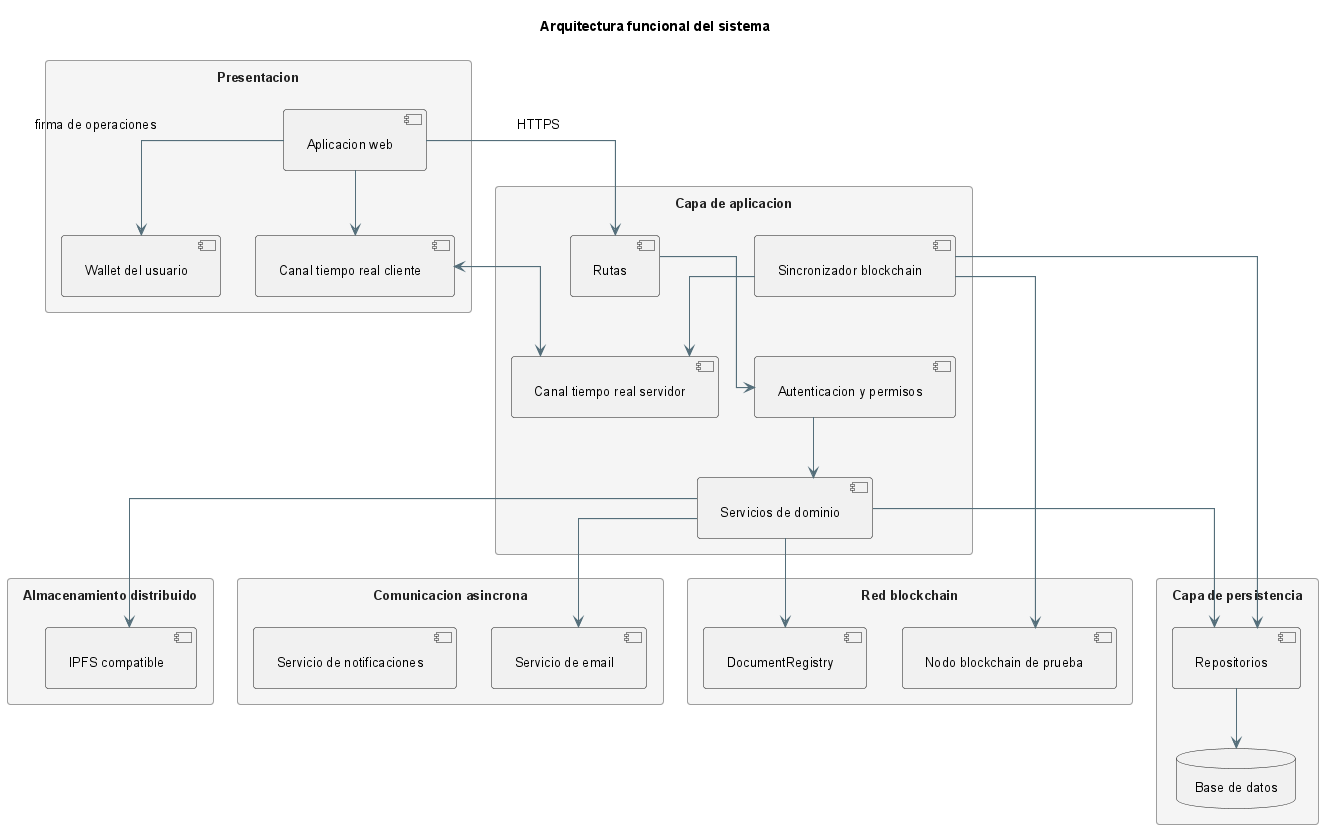
\includegraphics[width=0.85\textwidth]{diagramas/arquitectura.png}
    \caption{Arquitectura de cifrado de tres capas}
    \label{fig:cifrado}
\end{figure}

La Figura~\ref{fig:cifrado} ilustra el flujo completo: el usuario se autentica (Capa 1), el archivo se cifra con una clave unica que a su vez se protege con criptografia asimetrica (Capa 2), y finalmente se registra el hash del contenido cifrado en la blockchain (Capa 3).

\section{Integracion de capas de persistencia}

El sistema no podria operar unicamente con blockchain, ni tendria sentido construirlo solo sobre una base de datos relacional si se desea una huella de integridad externa. La arquitectura se apoya en tres capas de persistencia complementarias que conforman el denominado \textit{triangulo de persistencia}.

\begin{table}[H]
    \centering
    \small
    \renewcommand{\arraystretch}{1.4}
    \begin{tabular}{@{}p{2.8cm}p{4.2cm}p{4.2cm}p{3.5cm}@{}}
    \toprule
    \textbf{Capa} & \textbf{Que almacena} & \textbf{Ventajas} & \textbf{Desventajas} \\
    \midrule
    PostgreSQL & Usuarios, sesiones, preferencias, metadatos, organizacion por carpetas y etiquetas, estados de sincronizacion, notificaciones y proyecciones de consulta. & Permite busquedas complejas, filtros, actualizacion frecuente y relaciones con bajo coste operativo. & No garantiza inmutabilidad ni verificacion externa. \\
    \addlinespace
    IPFS & Ficheros documentales y sus versiones, en claro o cifrados segun visibilidad. & Proporciona direccionamiento por contenido (CID) y separacion entre archivo binario y registro transaccional. & La disponibilidad depende del pinning; sin incentivos economicos, la persistencia no esta garantizada por la red publica. \\
    \addlinespace
    Blockchain & Identificador documental, CID, roles, firmas, cambios de titularidad y estados criticos del documento. & Aporta inmutabilidad, trazabilidad compartida y posibilidad de verificacion independiente sin confianza en un tercero. & Coste de gas, latencia elevada, capacidad de almacenamiento limitada y rigidez en las modificaciones. \\
    \bottomrule
    \end{tabular}
    \caption{Reparto de responsabilidades entre las tres capas de persistencia}
    \label{tab:capas-persistencia}
\end{table}

Ese reparto evita dos extremos poco convenientes. Si todo se conservara en PostgreSQL, la aplicacion seria mas simple pero perderia la dimension de evidencia externa que justifica el proyecto. Si todo se intentara llevar a Ethereum, el sistema resultaria costoso, rigido y tecnicamente desproporcionado para el tipo de operaciones que se ejecutan a diario.

\subsection{Funcionamiento de IPFS}

IPFS se emplea como capa de almacenamiento distribuido mediante un adaptador configurable en backend. En funcion del entorno, puede utilizarse un nodo Kubo autoalojado o un proveedor gestionado como Pinata, manteniendo en ambos casos direccionamiento por contenido basado en CID.

Cada archivo subido genera un \textit{Content Identifier} (CID). Ese identificador depende del contenido y no de una ruta logica decidida por la aplicacion. Cuando el documento cambia, aunque solo se altere un byte, se obtiene un CID distinto. Esa propiedad encaja de forma natural con el versionado documental: cada version activa o restaurada queda asociada a un CID concreto, y la cadena registra precisamente esa referencia inmutable.

El tratamiento del archivo depende de la visibilidad documental. Si el documento es privado, el backend recibe el fichero en bruto, lo cifra con AES-256-GCM, sube a IPFS el resultado cifrado y almacena en la base de datos la clave simetrica cifrada, el vector de inicializacion y la etiqueta de autenticacion. Si el documento es publico, no se aplica ese cifrado del binario y el archivo se conserva en claro.

\subsection{Flujo de lectura/escritura coordinado}

Las operaciones de lectura y escritura atraviesan las tres capas de forma coordinada:

\textbf{Escritura.} El backend recibe el archivo, lo persiste temporalmente en disco, lo cifra si es necesario, lo sube a IPFS, obtiene el CID, crea el registro en PostgreSQL con estado \texttt{PREPARING} y, tras la confirmacion blockchain, actualiza el estado a \texttt{SYNCED}.

\textbf{Lectura.} El backend consulta PostgreSQL para recuperar los metadatos y la clave cifrada; solicita el contenido al nodo IPFS mediante el CID; descifra la clave simetrica con la clave privada del usuario; y finalmente descifra el archivo con AES-256-GCM antes de enviarlo al cliente.

\section{Smart contract consolidado DocumentRegistry}

La implementacion actual se concentra en un unico contrato, \texttt{DocumentRegistry}, situado en \texttt{smart-contracts/contracts/DocumentRegistry.sol}. Se trata de un contrato consolidado que integra registro de documentos, versionado, firmas y control de acceso.

Para soportar esa logica se utilizan utilidades de OpenZeppelin. \texttt{AccessControl} permite diferenciar roles administrativos globales; \texttt{ReentrancyGuard} limita ataques por reentrada; y \texttt{EnumerableSet} mantiene colecciones de documentos y usuarios con operaciones de consulta razonables.

\subsection{Estructuras de datos on-chain}

El contrato se apoya en tres \textit{structs} principales y en varios \textit{mappings} anidados.

\begin{table}[H]
    \centering
    \small
    \renewcommand{\arraystretch}{1.4}
    \begin{tabular}{@{}p{3.3cm}p{4.2cm}p{6.9cm}@{}}
    \toprule
    \textbf{Elemento} & \textbf{Campos principales} & \textbf{Funcion dentro del sistema} \\
    \midrule
    \texttt{Document} & \parbox[t]{4.1cm}{\texttt{docId}, \texttt{owner},\\ \texttt{createdAt}, \texttt{updatedAt},\\ \texttt{currentVersion}, \texttt{latestVersion},\\ \texttt{isArchived}, \texttt{isDeleted}} & Representa el estado documental minimo que debe mantenerse en cadena: titularidad, version operativa y marcas de estado. \\
    \addlinespace
    \texttt{Version} & \parbox[t]{4.1cm}{\texttt{versionNumber}, \texttt{ipfsCid},\\ \texttt{encryptedKeyHash}, \texttt{createdBy},\\ \texttt{createdAt}, \texttt{isOperational},\\ \texttt{restoredFrom}} & Vincula cada version con su CID de IPFS y reserva un campo para asociar metadatos criptograficos sin exponer la clave real. \\
    \addlinespace
    \texttt{Signature} & \parbox[t]{4.1cm}{\texttt{signer}, \texttt{signature},\\ \texttt{message}, \texttt{comment},\\ \texttt{timestamp}} & Registra la evidencia de firma por direccion Ethereum, preservando el mensaje y el instante en el que se acepto la firma. \\
    \addlinespace
    \texttt{\_permissions} & \parbox[t]{4.1cm}{\texttt{docId} $\rightarrow$ \texttt{address}\\ $\rightarrow$ \texttt{DocumentRole}} & Determina el nivel de acceso efectivo de cada cuenta sobre cada documento. \\
    \bottomrule
    \end{tabular}
    \caption{Estructuras de datos principales del contrato \texttt{DocumentRegistry}}
    \label{tab:estructuras-solidity}
\end{table}

\subsection{Operaciones registradas en cadena}

Las funciones publicas del contrato reproducen el nucleo funcional del sistema documental. La Tabla~\ref{tab:funciones-contrato} resume las operaciones principales, sus parametros y los eventos asociados.

\begin{table}[H]
    \centering
    \small
    \renewcommand{\arraystretch}{1.4}
    \begin{tabular}{@{}p{4.2cm}p{4.8cm}p{4.8cm}@{}}
    \toprule
    \textbf{Funcion} & \textbf{Parametros principales} & \textbf{Eventos emitidos} \\
    \midrule
    \texttt{createDocument} & \texttt{docId}, \texttt{ipfsCid}, \texttt{encryptedKeyHash} & \texttt{DocumentCreated} \\
    \texttt{createVersion} & \texttt{docId}, \texttt{ipfsCid}, \texttt{encryptedKeyHash} & \texttt{VersionCreated} \\
    \texttt{restoreVersion} & \texttt{docId}, \texttt{versionNumber} & \texttt{VersionRestored} \\
    \texttt{setOperationalVersion} & \texttt{docId}, \texttt{versionNumber} & \texttt{OperationalVersionChanged} \\
    \texttt{shareDocument} & \texttt{docId}, \texttt{user}, \texttt{role} & \texttt{DocumentShared} \\
    \texttt{revokePermission} & \texttt{docId}, \texttt{user} & \texttt{PermissionRevoked} \\
    \texttt{signDocument} & \texttt{docId}, \texttt{signature}, \texttt{message} & \texttt{DocumentSigned} \\
    \texttt{transferOwnership} & \texttt{docId}, \texttt{newOwner} & \texttt{OwnershipTransferred} \\
    \texttt{setArchiveStatus} & \texttt{docId}, \texttt{isArchived} & \texttt{DocumentArchived} \\
    \texttt{deleteDocument} & \texttt{docId} & \texttt{DocumentDeleted} \\
    \bottomrule
    \end{tabular}
    \caption{Funciones publicas y eventos del contrato consolidado}
    \label{tab:funciones-contrato}
\end{table}

A continuacion se detalla el proposito de cada operacion:

\begin{itemize}
    \item \texttt{createDocument}: crea el documento inicial, registra la primera version y concede al emisor el rol \texttt{OWNER}.
    \item \texttt{createVersion}: anade una nueva version, desactiva la version operativa previa y actualiza el contador.
    \item \texttt{restoreVersion}: genera una version nueva reutilizando el CID y el hash criptografico de una version anterior.
    \item \texttt{setOperationalVersion}: permite senalar otra version ya existente como operativa.
    \item \texttt{shareDocument} y \texttt{revokePermission}: gestionan permisos de lectura y edicion para terceros.
    \item \texttt{signDocument}: registra firmas verificables por version y evita duplicados.
    \item \texttt{transferOwnership}: transfiere la titularidad del documento y reajusta los roles del propietario saliente y del entrante.
    \item \texttt{setArchiveStatus} y \texttt{deleteDocument}: expresan archivado y borrado logico sin eliminar el rastro historico ya publicado.
\end{itemize}

\subsection{Eventos y restricciones de seguridad}

Cada operacion emite eventos que constituyen la interfaz de auditoria natural del sistema. \texttt{DocumentCreated} y \texttt{VersionCreated} registran altas y versionados; \texttt{DocumentShared} y \texttt{PermissionRevoked} reflejan cambios de permisos; \texttt{DocumentSigned} deja constancia de la firma emitida por una direccion concreta.

Las restricciones de seguridad se expresan mediante modificadores y controles internos. \texttt{nonReentrant} reduce la superficie de ataques por reentrada; \texttt{notDeleted} bloquea acciones incompatibles con el borrado logico; y \texttt{notArchived} impide modificar el estado de documentos archivados. El contrato conserva ademas salvaguardas defensivas adicionales a nivel interno, pero no se documentan como funcionalidades visibles del sistema final.

\section{Patron prepare/confirm y sincronizacion}

Las operaciones que modifican el estado documental y requieren evidencia on-chain no se ejecutan en un unico paso, porque la firma de la transaccion debe realizarse con la clave privada del usuario, que nunca abandona su wallet.

\textbf{Fase prepare.} Cuando el usuario solicita crear un documento, una version o una firma, el backend realiza todo aquello que no requiere firma blockchain: valida permisos, cifra el binario con AES-256-GCM cuando el documento es privado, sube el resultado a IPFS, genera los identificadores necesarios y crea un registro en PostgreSQL con estado \texttt{PREPARING}.

\textbf{Fase confirm.} El frontend usa esos datos para construir la transaccion, la firma con la wallet del usuario y la envia a la red. Una vez que dispone del \textit{transaction hash}, llama al endpoint de confirmacion del backend. Este endpoint recibe el hash y el identificador blockchain, localiza el registro previamente preparado y actualiza su estado a \texttt{TX\_SUBMITTED}.

\textbf{Sincronizacion final.} Un trabajador periodico (\texttt{blockchainSync.ts}) consulta cada cinco minutos los registros en estado \texttt{TX\_SUBMITTED} y pide el \textit{receipt} de cada transaccion al proveedor Ethereum. Si el \textit{receipt} indica exito (\texttt{status === 1}), el registro pasa a \texttt{SYNCED}. Si la transaccion fue revertida (\texttt{status === 0}), el estado cambia a \texttt{FAILED}.

El pseudocodigo detallado de estas fases se presento en la List~\ref{lst:prepare-confirm}. La separacion de responsabilidades entre fases permite que el frontend se mantenga agnostico respecto a la logica de negocio, mientras que el backend no requiere acceso a las claves privadas de los usuarios.

\section{Observabilidad blockchain y sincronizacion de estado}

\subsection{El patron de observabilidad mediante Event Listener}

Una de las decisiones arquitectonicas mas relevantes del sistema es que el backend \textbf{no consulta la blockchain para cada operacion de lectura}. En su lugar, mantiene una copia sincronizada del estado on-chain en PostgreSQL, actualizada mediante un mecanismo de observabilidad basado en eventos de Solidity.

El componente encargado de esta sincronizacion es el \texttt{Event Listener}, implementado en \texttt{backend/src/services/blockchainSync.ts}. Su funcionamiento sigue el siguiente ciclo:

\begin{enumerate}
    \item \textbf{Escucha de eventos.} Al arrancar el backend, el \texttt{Event Listener} se suscribe a todos los eventos definidos en el contrato \texttt{DocumentRegistry}: \texttt{DocumentCreated}, \texttt{VersionCreated}, \texttt{DocumentShared}, \texttt{PermissionRevoked}, \texttt{DocumentSigned}, \texttt{OwnershipTransferred}, \texttt{DocumentArchived}, \texttt{DocumentDeleted}, etc.
    \item \textbf{Procesamiento en tiempo real.} Cuando el minero confirma un bloque que contiene una transaccion del sistema, el nodo Ethereum emite el evento correspondiente. El listener lo captura, extrae sus parametros (identificador de documento, direccion del usuario, nuevo rol, CID, etc.) y actualiza inmediatamente el registro en PostgreSQL.
    \item \textbf{Sincronizacion periodica.} Ademas del canal de eventos en tiempo real, un trabajador periodico (cada cinco minutos) recorre los registros en estado \texttt{TX\_SUBMITTED} que aun no han sido confirmados por la via de eventos. Para cada uno, consulta el \textit{receipt} de la transaccion al proveedor Ethereum. Si el \textit{receipt} indica exito (\texttt{status === 1}), el registro pasa a \texttt{SYNCED}. Si fue revertida (\texttt{status === 0}), se marca como \texttt{FAILED}.
    \item \textbf{Tolerancia a fallos.} Si el listener pierde la conexion con el nodo Ethereum o el backend se reinicia, el trabajador periodico garantiza que los eventos emitidos durante la ventana de desconexion se recuperen consultando los bloques desde el ultimo bloque procesado.
\end{enumerate}

Este diseno ofrece dos ventajas fundamentales. Primero, las lecturas de metadatos, listados de documentos y consultas de permisos se resuelven contra PostgreSQL, con la latencia y la flexibilidad de consulta de una base de datos relacional. Segundo, la blockchain funciona como fuente de verdad auditada: cualquier discrepancia entre el estado en PostgreSQL y el estado on-chain puede detectarse cotejando los eventos historicos.

\subsection{Flujo completo de una operacion documental}

Para ilustrar la coordinacion entre las tres capas (frontend, backend y blockchain), se describe a continuacion el flujo de creacion de un documento privado con firma, que constituye la operacion mas representativa del sistema:

\begin{enumerate}
    \item \textbf{Subida del archivo.} El usuario selecciona un archivo y metadatos en la interfaz. El frontend envia el binario al backend mediante una peticion HTTP multipart.
    \item \textbf{Cifrado y almacenamiento.} El backend genera una clave simetrica AES-256-GCM aleatoria, cifra el archivo con ella, y sube el resultado cifrado a IPFS. Obtiene el CID.
    \item \textbf{Preparacion de la transaccion.} El backend crea un registro en PostgreSQL con estado \texttt{PREPARING}, cifra la clave simetrica con la clave publica del usuario (ECDH P-256), y devuelve al frontend los datos necesarios para construir la transaccion blockchain.
    \item \textbf{Firma del usuario.} El frontend presenta los datos a la wallet del usuario (Metamask o WalletConnect). El usuario revisa y firma la transaccion.
    \item \textbf{Confirmacion.} El frontend envia el \textit{transaction hash} al backend. El backend marca el registro como \texttt{TX\_SUBMITTED}.
    \item \textbf{Sincronizacion on-chain.} El \texttt{Event Listener} detecta el evento \texttt{DocumentCreated} en el siguiente bloque. El backend actualiza el estado del documento a \texttt{SYNCED} y la interfaz del usuario refleja el cambio mediante WebSocket.
\end{enumerate}

Este flujo garantiza tres propiedades criticas: el archivo nunca viaja sin cifrar fuera del control del backend, la clave privada del usuario nunca abandona su wallet, y la evidencia de la operacion queda registrada en la blockchain de forma inmutable.

\section{Gestion de contraseñas, frases de recuperacion y claves}

\subsection{Derivacion de claves con Argon2}

El sistema utiliza el algoritmo \textbf{Argon2id} (ganador del Password Hashing Competition) para derivar claves a partir de la contraseña del usuario. Argon2id combina las variantes Argon2i (resistente a \textit{side-channel attacks}) y Argon2d (resistente a ataques GPU), ofreciendo proteccion equilibrada frente a ambos vectores.

Cuando el usuario se registra, el backend genera una sal aleatoria de 32 bytes y aplica Argon2id con los siguientes parametros: \texttt{memoryCost = 65536 KB}, \texttt{timeCost = 3} iteraciones, \texttt{parallelism = 4} hilos. El hash resultante se almacena en la tabla \texttt{User} de PostgreSQL. La contraseña en texto plano nunca se conserva en disco ni en memoria mas alla del tiempo necesario para completar el proceso de derivacion.

\subsection{Cifrado de claves privadas con frase de recuperacion}

La clave privada de cada usuario (utilizada para el intercambio ECDH en la capa de cifrado de documentos) se protege mediante un mecanismo adicional. La clave se cifra con AES-256-GCM utilizando una clave derivada de la frase de recuperacion del usuario. Esta frase de recuperacion se genera durante el registro y se muestra al usuario una unica vez, instandole a guardarla de forma segura.

Esta separacion entre la contraseña de acceso (que puede cambiarse) y la frase de recuperacion (que es inmutable y custodia la clave privada) sigue el principio de minimo privilegio. Si un atacante compromete la contraseña del usuario, aun necesitaria la frase de recuperacion para descifrar los documentos, ya que la clave privada necesaria para el intercambio ECDH permanece cifrada con esa segunda capa de proteccion.

\section{Despliegue tecnico con Docker}

La materializacion operativa de esta arquitectura se apoya en Docker Compose. El motivo principal no es unicamente la comodidad de arranque, sino la necesidad de conservar una topologia estable entre servicios que dependen unos de otros: PostgreSQL para persistencia relacional, Hardhat como red EVM local, backend Node.js para la logica de aplicacion, frontend servido por Nginx, Postfix para correo transaccional y un nodo Kubo para almacenamiento distribuido.

\subsection{Arquitectura de contenedores}

La Figura~\ref{fig:deployment} muestra la arquitectura de contenedores y sus interdependencias. Cada servicio se ejecuta en su propio contenedor aislado, comunicandose mediante una red virtual interna gestionada por Docker Compose.

\begin{figure}[H]
    \centering
    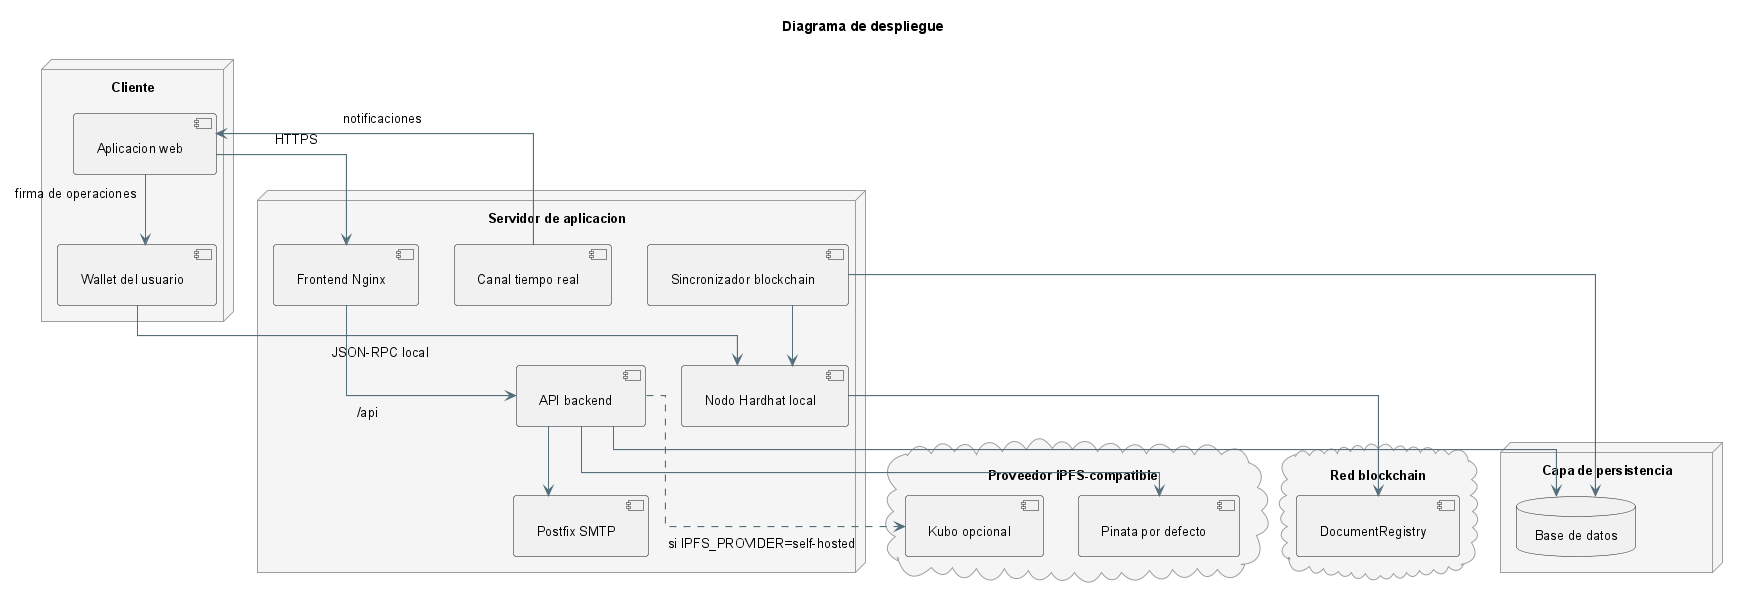
\includegraphics[width=0.95\textwidth]{diagramas/deployment.png}
    \caption{Arquitectura de despliegue con contenedores Docker}
    \label{fig:deployment}
\end{figure}

\subsection{Servicios del docker-compose}

El fichero \texttt{docker-compose.yml} define los siguientes servicios:

\begin{itemize}
    \item \textbf{postgres:} Base de datos relacional PostgreSQL 16. Almacena metadatos, usuarios, sesiones, estados de sincronizacion y claves cifradas. Expone el puerto 5432 internamente.
    \item \textbf{ipfs-node:} Nodo Kubo oficial de IPFS. Gestiona el almacenamiento distribuido de archivos, el pinning local y la API HTTP en el puerto 5001. Su volumen persistente garantiza que los CIDs no se pierdan ante reinicios.
    \item \textbf{hardhat:} Red Ethereum local para desarrollo y pruebas. Se ejecuta con la configuracion por defecto de Hardhat (cuentas pre-fundidas, minado automatico). Expone el RPC en el puerto 8545.
    \item \textbf{backend:} Servicio Node.js que encapsula la API REST. Depende de \texttt{postgres} e \texttt{ipfs-node}. Se reconstruye automaticamente ante cambios en el codigo fuente durante el desarrollo.
    \item \textbf{frontend:} Imagen de produccion basada en Nginx. Sirve los assets estaticos generados por Vite y redirige las rutas de la SPA al fichero \texttt{index.html}.
    \item \textbf{nginx:} Proxy inverso que expone los puertos 80 y 443 hacia el exterior. Redirige las peticiones a \texttt{/api} al backend y el resto al contenedor del frontend. Termina las conexiones SSL/TLS cuando se configuran certificados.
    \item \textbf{postfix:} Servidor de correo para el envio de notificaciones transaccionales (verificacion de cuenta, recuperacion de acceso) sin depender de servicios SMTP externos.
\end{itemize}

\subsection{Volúmenes, redes y variables de entorno}

\textbf{Volúmenes.} Se definen volúmenes Docker persistentes para \texttt{postgres-data} (ficheros de base de datos), \texttt{ipfs-data} (repositorio de bloques y configuracion del nodo Kubo) y \texttt{backend-logs} (ficheros de trazas de Winston). Esta separacion garantiza que los datos sobrevivan a la recreacion de contenedores.

\textbf{Redes.} Todos los servicios se conectan a una red bridge interna denominada \texttt{documentchain-network}. El aislamiento de red impide que servicios externos accedan directamente a PostgreSQL o al API de IPFS sin pasar por Nginx y el backend.

\textbf{Variables de entorno.} La configuracion sensible (claves JWT, credenciales de base de datos, URL del nodo Ethereum) se inyecta mediante un fichero \texttt{.env} que no se versiona en el repositorio. Durante el despliegue mediante GitHub Actions, estas variables se configuran como secretos del repositorio.

\subsection{Integracion continua (CI/CD)}

El proyecto incorpora un \textit{workflow} de \textit{GitHub Actions} orientado a \textit{runners} autoalojados en Linux. Cuando llega un \textit{push} a la rama principal, el pipeline ejecuta las siguientes fases:

\begin{enumerate}
    \item \textbf{Checkout y dependencias.} Clona el repositorio e instala las dependencias de frontend, backend y smart contracts.
    \item \textbf{Tests.} Ejecuta los tests unitarios con Vitest (frontend), Jest (backend) y Hardhat (smart contracts). Si algun test falla, el pipeline se interrumpe.
    \item \textbf{Build.} Compila el frontend para produccion, transpila el backend y genera los artefactos de despliegue.
    \item \textbf{Despliegue.} El \textit{runner} autoalojado actualiza el codigo en el servidor, reconstruye las imagenes Docker necesarias, aplica las migraciones Prisma pendientes y reinicia los servicios mediante Docker Compose.
\end{enumerate}

Una decision arquitectonica explicita del proyecto es no utilizar un patron de proxy upgradeable para el contrato inteligente. Aunque los proxies permiten actualizar la logica sin cambiar su direccion, su implementacion anade complejidad adicional. En este trabajo se ha priorizado la claridad del codigo y la reproducibilidad del entorno de pruebas. Como consecuencia, cualquier modificacion en \texttt{DocumentRegistry} exige un redeploy completo. El script \texttt{reseed-dev.ps1} automatiza precisamente ese ciclo.

\section{Glosario tecnico}

\begin{description}
    \item[ABI] Application Binary Interface, interfaz que define como interactuar con un smart contract desde codigo externo.
    \item[AES-256-GCM] Advanced Encryption Standard en modo Galois/Counter Mode con clave de 256 bits. Proporciona confidencialidad y autenticacion simultaneas.
    \item[Argon2] Algoritmo de derivacion de claves ganador del Password Hashing Competition, resistente a ataques de paralelizacion en GPU.
    \item[CID] Content Identifier, identificador unico de contenido en IPFS basado en hash criptografico.
    \item[ECDH] Elliptic Curve Diffie-Hellman, protocolo de intercambio de claves sobre curvas elipticas que permite acordar un secreto compartido de forma segura.
    \item[EVM] Ethereum Virtual Machine, entorno de ejecucion de smart contracts en redes compatibles con Ethereum.
    \item[Event Listener] Servicio del backend que escucha eventos emitidos por el smart contract para sincronizar estados.
    \item[Gas] Unidad de medida del coste computacional de operaciones en la EVM; se paga en la moneda nativa de la red.
    \item[Hardhat] Entorno de desarrollo, testing y despliegue de smart contracts en la EVM.
    \item[IPFS] InterPlanetary File System, protocolo y red de almacenamiento distribuido por contenido.
    \item[JWT] JSON Web Token, estandar compacto y autocontenido para la transmision segura de informacion entre partes.
    \item[Kubo] Implementacion oficial de nodo IPFS desarrollada en Go; se usa en el proyecto para almacenamiento autoalojado.
    \item[Mapping] Estructura de datos tipo diccionario en Solidity que relaciona claves con valores.
    \item[Metamask] Billetera digital de navegador que permite gestionar claves privadas e interactuar con aplicaciones descentralizadas.
    \item[NatSpec] formato de documentacion embebida en comentarios de Solidity para generar especificaciones legibles por maquina.
    \item[Pinning] Accion de mantener contenido permanentemente disponible en un nodo IPFS, evitando que sea eliminado por el recolector de basura.
    \item[Prisma] ORM de siguiente generacion para Node.js y TypeScript que proporciona tipado seguro y migraciones.
    \item[Reentrancia] Vulnerabilidad por la que una funcion externa puede ser llamada repetidamente antes de que termine la ejecucion original; mitigada con \texttt{ReentrancyGuard}.
    \item[Sepolia] Red de pruebas publica de Ethereum utilizada para validar contratos antes de un despliegue en mainnet.
    \item[shadcn/ui] Coleccion de componentes React reutilizables construidos sobre Radix UI y Tailwind CSS.
    \item[TxHash] Transaction Hash, identificador unico de una transaccion confirmada en blockchain.
    \item[UML] Unified Modeling Language, lenguaje grafico estandar para la especificacion, visualizacion y documentacion de sistemas software.
    \item[Vite] Herramienta de construccion frontend que utiliza ES Modules nativos para un desarrollo rapido.
    \item[WalletConnect] Protocolo abierto que permite conectar wallets moviles con aplicaciones descentralizadas mediante codigos QR.
\end{description}

\section{Conclusiones del Anexo IV}

El presente anexo ha documentado la totalidad del codigo fuente del sistema DocumentChain, incluyendo las tecnologias empleadas, la estructura modular del proyecto, los metodos criticos de cifrado y sincronizacion, los smart contracts principales, la arquitectura de cifrado de tres capas, el reparto de responsabilidades entre PostgreSQL, IPFS y blockchain, el patron prepare/confirm y el despliegue mediante Docker.

Se ha prestado especial atencion a la reproducibilidad del entorno, la trazabilidad de las decisiones de diseno y la separacion de responsabilidades entre capas. La documentacion tecnica aqui presentada constituye la referencia definitiva para cualquier desarrollador que deba mantener o extender el sistema, asi como para auditores que requieran comprender los flujos de cifrado, sincronizacion y control de acceso sin necesidad de reconstruir la logica a partir del codigo fuente exclusivamente.

\end{document}
